%%*************************************************************************
%% Helga Ingimundardottir, hei2@hi.is
%% LaTeX source code for LION6
%%   Problem difficulty in JSSP
%%
%% File list of work: lion6.tex, lion6.bib, lion6.ps, lion6.pdf, 
%% and figures figs/***.eps
%%                    
%%*************************************************************************
%% NOTE: ps2pdf -dEmbedAllFonts=true -dSubsetFonts=true -dEPSCrop=true -dPDFSETTINGS=/prepress lion6.ps

%\documentclass[10pt, conference, compsocconf]{IEEEtran} 
\documentclass[10pt]{llncs} % so paper is more compact
% Add the compsocconf option for Computer Society conferences.

% *** CITATION PACKAGES ***
\usepackage{cite}

% *** GRAPHICS RELATED PACKAGES ***
\usepackage[dvips]{graphicx}
% declare the path(s) where your graphic files are
\graphicspath{{figs/}}
% and their extensions so you won't have to specify these with
% every instance of \includegraphics
\DeclareGraphicsExtensions{.eps}

% *** MATH PACKAGES ***
\usepackage{latexsym}
\usepackage[cmex10]{amsmath}\usepackage{amssymb}
% Also, note that the amsmath package sets \interdisplaylinepenalty to 10000
% thus preventing page breaks from occurring within multiline equations. Use:
\interdisplaylinepenalty=2500

% *** ALIGNMENT PACKAGES ***
\usepackage{tabularx}


% *** Helga's math-shorthand ***
\newcommand{\inner}[2]{\big<{#1}\cdot{#2}\big>}
\renewcommand{\vec}[1]{{\mbox{\boldmath$#1$}}}
\newcommand{\hard}{\emph{hard} }
\newcommand{\easy}{\emph{easy} }
\newcommand{\good}{\emph{good} }
\newcommand{\bad}{\emph{bad} }

% correct bad hyphenation here
\hyphenation{op-tical net-works semi-conduc-tor}


\begin{document}
% paper title
% can use linebreaks \\ within to get better formatting as desired
\title{Determining the Characteristic of Difficult Job Shop Scheduling Instances for a Heuristic Solution Method}

\author{Helga Ingimundardottir \and Thomas Philip Runarsson}
\institute{{School of Engineering and Natural Sciences, University of Iceland}\\
\email{hei2@hi.is} and \email{tpr@hi.is}}


% make the title area
\maketitle

\begin{abstract} 
Many heuristic methods have been proposed for the job-shop scheduling problem. Different solution methodologies outperform other depending on the particular problem instance under consideration. Therefore, one is interested in knowing how the instances differ in structure and determine when a particular heuristic solution is likely to fail and explore in further detail the causes. In order to achieve this, we seek to characterise features for different difficulties. Preliminary experiments show there are different significant features that distinguish between easy and hard JSSP problem, and that they vary throughout the scheduling process. 
The insight attained by investigating the relationship between problem structure and heuristic performance can undoubtedly lead to better heuristic design that is tailored to the data distribution under consideration.
\end{abstract}

%\begin{IEEEkeywords}
%scheduling; job shop; problem difficulty; performance prediction; knowledge discovery
%\end{IEEEkeywords}

\section{Introduction}\label{sec:introduction}
Hand crafting heuristics for NP-hard problems is a time-consuming trial and error process, requiring inductive reasoning or problem specific insights from their human designers. Furthermore, within a problems class, such as job-shop scheduling, it is possible to construct problem instances where one heuristic would outperform another. 
Depending on the underlying data distribution, different heuristics perform differently, commonly known as the \emph{no free lunch} theorem \cite{WoMa97:tec}. The success of a heuristic is how it manages to deal with and manipulate the characteristics of its given problem instance. So in order to understand more fully how a heuristic will eventually perform, one needs to look into what kind of problem instances are being introduced to the system. What defines a problem instance, e.g. what are its key features? And how can they help with designing better heuristics?

%A common and simple way of finding a good feasible solution for the JSSP is by applying heuristic dispatching rules. , e.g., choosing a task corresponding to longest/shortest operation time;  most/least successors; or ranked positional weight, i.e., sum of operation times of its predecessors. Ties are broken in an arbitrary fashion or by another heuristic rule. There is no dominant rule for JSSP, but the most effective have been: most work remaining (MWRM); least work remaining (LWKR); shortest processing time (SPT); and longest processing time (LPT). The classical dispatching rules are continually used in research, and for this study only MWRM will be explored.

In investigating the relationship between problem structure and heuristic effectiveness one can research what \cite{Corne2011} calls \emph{footprints} in instance space, which is an indicator how an algorithm generalises over the instance space. This sort of investigation has also been referred to as \emph{landmarking} \cite{Pfahringer2000}. 
% quote Corne2011: ``such a footprint indicates how an algorithm's comparative performance generalises in instance space''
% quote Katie2009: ``Landmarking tries to directly characterise a domain by relating the performance to some learners -- the landmarkers -- to the performance of some other algorithm.''
It is evident from experiments performed in \cite{Corne2011} that one-algorithm-for-all problem instances is not ideal. An algorithm may be favoured for its best overall performance, however it was rarely the best algorithm available over various subspaces of the instance space.
Thus when comparing different algorithms one needs to explore how they perform w.r.t. the instance space, i.e. their footprint. %That is to say, one can look at it as finding what footprints correspond to a subset of the instance space that works \emph{well} for a given algorithm, and similarly finding what footprints correspond to a subset of the instance space that works \emph{poorly} for a given algorithm. In this study this corresponds to finding \good and \bad JSSP schedules, respectively. 

%In \cite{Smith-miles2010}, the authors also investigate algorithm performance in instance space using footprints. The main difference between \cite{Corne2011} and \cite{Smith-miles2010} is how they discretise the instance space. In the case of \cite{Corne2011} they use JSSP and discretise manually between different problem instances, on one hand w.r.t. processing times, e.g. $p\sim U(10,20)$ vs. $p\sim(20,30)$ etc, and on the other hand w.r.t. number of tasks $n$. They warn that footprinting can be uneven, so great care needs to be taken in how to discretise the instance space into subspaces. 
%For the timetabling instances in \cite{Smith-miles2010} a self-organizing map was used implemented to group similar problem instances together, that were both real world instances and synthetic ones using different problem generators. 
In this study, the same problem generator is used to create 1,500 problem instances, however the experimental study in section~\ref{sec:expr} shows that MWRM works well/poorly on a subset of the instances. Since the problem instances are only defined by processing times and its permutation, the interaction between the two is important, because it introduces hidden properties in the data structure making it easy or hard to schedule with for the given algorithm. These underlying characteristics or features define its data structure. So a sophisticated way of discretising the instance space is grouping together problem instances that show the same kind of feature behaviour, in order to infer what is the feature behaviour between \good and \bad schedules. 

It is interesting to know if the difference in the structure of the schedule is time dependent, is there a clear time of divergence within the scheduling process? Moreover, investigation of how sensitive is the difference between two sets of features, e.g. can two schedules with similar feature values yield completely contradictory outcomes, i.e. one poor and one good schedule? Or will they more or less follow the same path? This essentially answers the question of whether is is in fact feasible to discriminate between \good and \bad schedules using the currently selected features as a measure. If results are contradictory, it is an indicator the features selected are not robust enough to capture the essence of the data structure. 
Additionally, there is also the question of how can one define `similar' schedules, what measures should be used? This paper describes some preliminary experiments with the aim of investigating the feasibility of finding distinguishing features corresponding to \good and \bad schedules in JSSP.

Instead of searching through a large set of algorithms (creating an algorithm portfolio) and determining which algorithm is the most suitable for a given subset of the instance space, as is generally the focus in the current literature \cite{Smith-miles2009,Smith-miles2010,Corne2011}, our focus is rather on a single algorithm and understanding \emph{how} it works on the instance space -- in the hopes of being able to extrapolate where it excels in order to aid its failing aspects.

The outline of the paper is as follows, in section~\ref{sec:JSSP} priority dispatch rules for the JSSP problem are discussed, what features are of interest and how data is generated. %Followed by a discussion of how to map the relationship between problem structure and heuristic efficiency in section~\ref{sec:relationship}. 
A preliminary experimental study is presented in section~\ref{sec:expr}. The paper concludes with a summary of main findings and points to future work.

\section{Job-shop scheduling}\label{sec:JSSP}
The job-shop scheduling task considered here is where $n$ jobs are scheduled on a set of $m$ machines, subject to the constraint that each job must follow a predefined machine order and that a machine can handle at most one job at a time. 
The objective is to schedule the jobs so as to minimize the maximum completion times, also known as the makespan.  For a mathematical formulation of JSSP the reader is recommended \cite{Ingimundardottir2010}. 

\subsection{Single-priority dispatching heuristic}
Dispatching rules are of a construction heuristics, where one starts with an empty schedule and adds on one job at a time. When a machine is free the dispatching rule inspects the waiting jobs and selects the job with the highest priority. A survey of more than 100 of such priority rules was given in 1977 by \cite{Panwalkar1977a}. In this paper however, only most work remaining (MWRM) dispatching rule will be investigated.

In order to apply a dispatching rule a number of features of the schedule being built must be computed. The features of particular interest were obtained from inspecting the aforementioned single priority-based dispatching rules. The temporal scheduling features applied in this paper are given in Table~\ref{tbl:feat}. %Note that features 1--13 can be varying throughout the scheduling process  w.r.t. the tasks that can be dispatched next at that time point, whereas features 14--16 remain constant for a problem instance. 
These are not the only possible set of features, they are however built on the work published in \cite{Ingimundardottir2010,Smith-miles2009} and deemed successful in capturing the essence of a JSSP data structure.


%A dispatch rule may need to perform a one-step look-ahead and observes features of the partial schedule to make a decision, for example by observing the resulting temporal makespan. These resulting observed features are sometimes referred to as an \emph{after-state} or \emph{post-decision state}. %Other dispatch rules use features not directly observable from the current partial schedule, for example by assigning jobs with most total processing time remaining, i.e. MWRM. %{\it Other features of importance are the job's starting time $x_s(a,j)$; the time job $j$ will be released $x_f(a,j)$; and the new time machine $a$ will be free again, $x_{\textrm{mac}}(a,j)+p_{\textrm{mac}}(a,j)$; current makespan; sum of slacks; and slacks weighted by number of operations.}

%A job is placed at the earliest available time slot for its next machine. After each dispatch the schedule's current features are updated based on the partly finished schedule. 

\begin{table}[t!]
 {\tiny
 \begin{center}
  \begin{tabular}{|c|l|}
   \hline\hline
  $\vec{\phi}$ & Feature description \\ \hline
  $\phi_1$ & processing time for job on machine\\
  $\phi_2$ & start-time \\
  $\phi_3$ & end-time \\
  $\phi_4$ & when machine is next free \\
  $\phi_5$ & current makespan \\
  $\phi_6$ & work remaining \\
  $\phi_7$ & most work remaining \\
  $\phi_8$ & slack time for this particular machine \\
  $\phi_9$ & slack time for all machines \\
  $\phi_{10}$ & slack time weighted w.r.t. number of operations already assigned \\
  $\phi_{11}$ & time job had to wait\\
  $\phi_{12}$ & size of slot created by assignment \\
  $\phi_{13}$ & total processing time for job \\
  $\phi_{14}$ & total processing time for all jobs \\%, $\sum_{j\in J}\sum_{a\in M} p(j,a)$\\
  $\phi_{15}$ & mean processing time for all jobs \\%, $\frac{1}{n\cdot m}\phi(1)$\\
  $\phi_{16}$ & range of processing times over all jobs \\%, $\max_{j\in J, a\in M}\{p(j,a)\}-\min_{j\in J, a\in M}\{p(j,a)\}$ \\
   \hline\hline
  \end{tabular}
 \end{center}}
 \caption{Feature space $\mathcal{F}$ for JSSP. Features 1--13 can vary throughout the scheduling process w.r.t. tasks that can be dispatched next, however features 14--16 are static.}
 \label{tbl:feat}
\end{table}

\subsection{Data generation}

Problem instances were generated stochastically by fixing the number of jobs and machines and sampling a discrete processing time from the uniform distribution $U(1,200)$. The machine order is a random permutation of $\{1,...,m\}$. A total of 1,500 instances were generated for a six job and six machine job-shop problem. 

%When building a complete schedule $n\times m$ dispatches must be made sequentially w.r.t. MWRM. We deliberately create a separate feature set for each dispatch iterations. %, as our initial feeling is that key features in the beginning of the schedule building process may not necessarily be the same as in the middle or end of the schedule. 
%Note that the features are not calculated for the last step, since that step is default and no heuristic involved. 

In the experimental study the performance of the MWRM, $\mu_{\text{MWRM}}$, and compared with its optimal makespan, $\mu_{\text{opt}}$. Since the optimal makespan varies between problem instances the following performance measure is used:
\begin{equation}\label{eq:ratio}\rho=\frac{\mu_{\text{MWRM}}}{\mu_{\text{opt}}}.\end{equation}


%\section{Relationship between problem structure and heuristic efficiency}\label{sec:relationship}



\section{Experimental study}\label{sec:expr}
In order to differentiate between problems, a threshold of a $\rho<1.1$ and $\rho>1.3$ was used to classify \easy and \hard problems.
Of the 1500 instances created, 271 and 161 problems were classified \easy and \hard\!, respectively.

%We are interested in knowing \emph{when} during the scheduling process \easy and \hard problems diverge and explore in further detail \emph{why} they diverged. %Hence a simple Kolmogorov-Smirnov goodness-of-fit hypothesis test with a significance level 0.05 is used to determine any statistical difference between data distribution of the features (on a step-by-step basis) between the \easy and \hard problem instances.
Table~\ref{tbl:feat:same} reports where data distributions are the same (denoted by $\cdot$).
From the table one can see that distribution for $\phi_1$, $\phi_6$, $\phi_{12}$ and $\phi_{16}$) are (more or less) the same throughout the scheduling process. 
However there is a clear time of divergence for distribution of slacks; step 6 for $\phi_8$ and step 12 for $\phi_9$ and $\phi_{10}$. 

\begin{table}[t!]
 {\tiny
 \begin{center}
 {\renewcommand{\arraystretch}{0.8} \renewcommand{\tabcolsep}{0.05cm} 
\begin{tabularx}{.9\columnwidth}{|X|ccccccccccccccccccccccccccccccccccc|}
\hline\hline
  & \multicolumn{35}{c|}{dispatch} \\ 
$\vec{\phi} $ & 1 & & 3 &  & 5  &  & 7 &  & 9 &   &11 & &13 & & 15  & &17 & &19 &   &21 & &23 & &25 & &27 & &29 &   &31 & &33 & & 35 \\ \hline 
$\phi_1$& $\bullet$ & $\bullet$ & $\bullet$ & $\bullet$ & $\bullet$ & $\bullet$ & $\bullet$ & $\bullet$ & $\bullet$ & $\bullet$ & $\bullet$ & $\bullet$ &   & $\bullet$ & $\bullet$ & $\bullet$ & $\bullet$ & $\bullet$ & $\bullet$ & $\bullet$ & $\bullet$ & $\bullet$ & $\bullet$ & $\bullet$ & $\bullet$ & $\bullet$ & $\bullet$ & $\bullet$ & $\bullet$ & $\bullet$ & $\bullet$ & $\bullet$ & $\bullet$ & $\bullet$ & $\bullet$ \\
$\phi_2$ & $\bullet$ &   & $\bullet$ &   &   &   & $\bullet$ &   &   &   &   &   &   &   &   &   &   &   &   &   &   &   &   &   &   &   &   &   &   &   &   &   &   &   &   \\
$\phi_3$ & $\bullet$ &   & $\bullet$ &   &   & $\bullet$ & $\bullet$ &   &   &   &   &   & $\bullet$ &   &   &   &   &   &   &   &   &   &   &   &   &   &   &   &   &   &   &   &   &   &  \\
$\phi_4$ & $\bullet$ &   &   &   &   &   & $\bullet$ &   &   &   &   &   &   &   &   &   &   &   &   &   &   &   &   &   &   &   &   &   &   &   &   &   &   &   &  \\
$\phi_5$ & $\bullet$ &   &   &   &   &   &   &   &   &   &   &   &   &   &   &   &   &   &   &   &   &   &   &   &   &   &   &   &   &   &   &   &   &   &  \\
$\phi_6$ & $\bullet$ &   &   & $\bullet$ & $\bullet$ &   &   & $\bullet$ &   & $\bullet$ & $\bullet$ & $\bullet$ & $\bullet$ & $\bullet$ & $\bullet$ & $\bullet$ & $\bullet$ & $\bullet$ & $\bullet$ & $\bullet$ & $\bullet$ & $\bullet$ & $\bullet$ & $\bullet$ & $\bullet$ & $\bullet$ & $\bullet$ & $\bullet$ & $\bullet$ & $\bullet$ & $\bullet$ & $\bullet$ & $\bullet$ & $\bullet$ & $\bullet$ \\
$\phi_7$ &   &   &   &   &   &   &   &   &   &   &   &   &   &   & $\bullet$ &   &   & $\bullet$ & $\bullet$ & $\bullet$ & $\bullet$ & $\bullet$ & $\bullet$ & $\bullet$ & $\bullet$ & $\bullet$ & $\bullet$ & $\bullet$ & $\bullet$ &   &   &   & $\bullet$ & $\bullet$ & $\bullet$\\
$\phi_8$ & $\bullet$ & $\bullet$ & $\bullet$ & $\bullet$ & $\bullet$ & $\bullet$ &   &   &   &   &   &   &   &   &   &   &   &   &   &   &   &   &   &   &   &   &   &   &   &   &   &   &   &   &  \\
$\phi_9$ & $\bullet$ & $\bullet$ & $\bullet$ & $\bullet$ & $\bullet$ & $\bullet$ & $\bullet$ & $\bullet$ & $\bullet$ & $\bullet$ & $\bullet$ & $\bullet$ &   &   &   &   &   &   &   &   &   &   &   &   &   &   &   &   &   &   &   &   &   &   &  \\
$\phi_{10}$ & $\bullet$ & $\bullet$ & $\bullet$ & $\bullet$ & $\bullet$ & $\bullet$ & $\bullet$ & $\bullet$ & $\bullet$ & $\bullet$ &   & $\bullet$ &   &   &   &   &   &   &   &   &   &   &   &   &   &   &   &   &   &   &   &   &   &   &  \\
$\phi_{11}$ & $\bullet$ & $\bullet$ & $\bullet$ &   & $\bullet$ & $\bullet$ & $\bullet$ &   &   & $\bullet$ & $\bullet$ & $\bullet$ &   & $\bullet$ & $\bullet$ &   & $\bullet$ & $\bullet$ &   & $\bullet$ & $\bullet$ &   &   &   &   &   &   & $\bullet$ & $\bullet$ &   &   &   &   &   &  \\
$\phi_{12}$ & $\bullet$ &   & $\bullet$ & $\bullet$ & $\bullet$ & $\bullet$ & $\bullet$ & $\bullet$ & $\bullet$ & $\bullet$ & $\bullet$ & $\bullet$ & $\bullet$ &   & $\bullet$ & $\bullet$ &   & $\bullet$ & $\bullet$ &   & $\bullet$ &   & $\bullet$ & $\bullet$ & $\bullet$ & $\bullet$ &   &   &   &   & $\bullet$ &   &   &   & $\bullet$\\
$\phi_{13}$ &   & $\bullet$ & $\bullet$ &   &   &   & $\bullet$ &   &   &   &   & $\bullet$ &   & $\bullet$ &   & $\bullet$ & $\bullet$ & $\bullet$ & $\bullet$ &   &   & $\bullet$ & $\bullet$ & $\bullet$ & $\bullet$ & $\bullet$ & $\bullet$ &   & $\bullet$ &   & $\bullet$ &   & $\bullet$ & $\bullet$ &  \\
$\phi_{14}$ &   &   &   &   &   &   &   &   &   &   &   &   &   &   &   &   &   &   &   &   &   &   &   &   &   &   &   &   &   &   &   &   &   &   &  \\
$\phi_{15}$ &   &   &   &   &   &   &   &   &   &   &   &   &   &   &   &   &   &   &   &   &   &   &   &   &   &   &   &   &   &   &   &   &   &   &  \\
$\phi_{16}$ & $\bullet$ & $\bullet$ & $\bullet$ & $\bullet$ & $\bullet$ & $\bullet$ & $\bullet$ & $\bullet$ & $\bullet$ & $\bullet$ & $\bullet$ & $\bullet$ & $\bullet$ & $\bullet$ & $\bullet$ & $\bullet$ & $\bullet$ & $\bullet$ & $\bullet$ & $\bullet$ & $\bullet$ & $\bullet$ & $\bullet$ & $\bullet$ & $\bullet$ & $\bullet$ & $\bullet$ & $\bullet$ & $\bullet$ & $\bullet$ & $\bullet$ & $\bullet$ & $\bullet$ & $\bullet$ & $\bullet$ \\
\hline\hline
\end{tabularx}}
 \end{center}}
 \caption{Features for \easy and \hard problems are drawn from the same data distribution (denoted by $\cdot$).}
 \label{tbl:feat:same}
\end{table}

In order to find defining characteristics for \easy and \hard problems, a (linear) correlation was computed between features (on a step-by-step basis) to the resulting ratio from optimality. Significant features are reported in Table~\ref{tbl:feat:easynhard} for \easy and \hard problems, (denoted by $\cdot$).
As one can see from the tables, the significant features for the different difficulties are varying. %Easy problems have considerably more relevant features than hard problems (total 133 vs. 63). 
Some are commonly significant features across the tables (denoted by $\bullet$). %Take for instance, current makespan, $\phi_5$, it is significant across (most of) the scheduling process for \easy problems. Whereas, it is only significant near the finishing stages in the case of \hard problems. 
%Since the heuristic being used to schedule is MWRM, it is counter-intuitive that the features corresponding to work remaining ($\phi_6$ and $\phi_7$) are not significant. Instead the slack of the machine, $\phi_8$, is more interesting indicator for a schedule. 

%\begin{table}[t!]
% {\footnotesize
% \begin{center}
%  \begin{tabular}{|l|c|lll|}
%  \hline\hline
%  & & \multicolumn{3}{|c|}{$\rho$} \\ 
%  & $\#$ & mean & min & max\\ \hline 
%  \easy & 271 & 1.06 & 1.00 & 1.10 \\ 
%  \hard & 161 & 1.35 & 1.30 & 1.51 \\ 
%   \hline\hline
%  \end{tabular}
% \end{center}}
% \caption{Main statistics for \easy and \hard problems.}
% \label{tbl:stats}
%\end{table}

\begin{table}[t!]
 {\tiny
 \begin{center}
 {\renewcommand{\arraystretch}{0.8} \renewcommand{\tabcolsep}{0.015cm} \tiny
\begin{tabularx}{.48\columnwidth}{|X|ccccccccccccccccccccccccccccccccccc|}
\hline\hline
Easy & \multicolumn{35}{c|}{dispatch} \\ 
${\phi}_i$  & 1 & &  &  & 5  &  &  &  &  & 10  & & & & & 15  & & & & & 20  & & & & & & && & & 30  & & & & & 35\\ \hline 
${1}$& &  &  &  &  &  &  &  &  &  &  &  &  &  &  &  &  &  &  &  &  &  &  &  &  &  &  &  &  &  &  &  &  &  & \\
${2}$& &  &  &  &  &  &  &  &  &  & $\bullet$ & $\bullet$ &  & $\cdot$ &  &  &  &  & $\cdot$ & $\cdot$ &  & $\cdot$ &  &  & $\cdot$ &  & $\bullet$ & $\bullet$ & $\cdot$ & $\cdot$ & $\cdot$ & $\bullet$ &  & $\cdot$ & $\bullet$ \\
${3}$& &  &  &  &  &  &  &  &  & $\cdot$ & $\bullet$ & $\cdot$ &  &  &  &  &  &  &  & $\cdot$ &  & $\cdot$ &  &  & $\cdot$ &  & $\bullet$ &  & $\cdot$ & $\cdot$ & $\cdot$ & $\bullet$ &  & $\cdot$ & $\bullet$ \\
${4}$& &  &  &  &  & $\cdot$ &  &  &  &  & $\bullet$ &  & $\bullet$ & $\cdot$ &  &  &  &  & $\cdot$ & $\cdot$ &  & $\cdot$ &  &  & $\cdot$ &  & $\bullet$ &  & $\cdot$ & $\cdot$ & $\bullet$ & $\bullet$ & $\bullet$ & $\cdot$ & $\cdot$ \\
${5}$& &  &  &  &  & $\cdot$ & $\cdot$ & $\cdot$ & $\cdot$ & $\cdot$ & $\cdot$ & $\bullet$ & $\bullet$ & $\cdot$ & $\cdot$ & $\cdot$ & $\cdot$ &  &  & $\cdot$ & $\cdot$ & $\bullet$ & $\cdot$ & $\cdot$ & $\bullet$ & $\cdot$ & $\bullet$ & $\bullet$ & $\bullet$ & $\bullet$ & $\bullet$ & $\bullet$ & $\bullet$ & $\bullet$ & $\bullet$ \\
${6}$& &  &  &  &  &  &  &  &  &  &  &  &  &  &  &  &  &  &  &  &  &  &  &  &  &  &  &  &  &  &  &  &  &  & \\
${7}$& &  &  &  &  &  &  &  &  &  &  &  &  &  &  &  &  &  &  &  &  &  &  &  &  &  &  &  &  &  &  &  &  &  & \\
${8}$& &  &  &  &  & $\cdot$ & $\cdot$ & $\cdot$ &  &  &  &  &  & $\cdot$ & $\cdot$ & $\cdot$ & $\cdot$ & $\bullet$ & $\bullet$ & $\bullet$ & $\bullet$ & $\cdot$ & $\cdot$ & $\cdot$ & $\cdot$ & $\cdot$ & $\cdot$ & $\bullet$ & $\bullet$ & $\bullet$ & $\cdot$ & $\bullet$ & $\cdot$ & $\cdot$ & $\bullet$ \\
${9}$& &  &  &  &  &  & $\cdot$ & $\cdot$ &  &  &  &  &  & $\cdot$ &  &  & $\cdot$ & $\cdot$ & $\cdot$ & $\cdot$ & $\bullet$ &  &  &  & $\cdot$ &  &  & $\bullet$ & $\cdot$ & $\cdot$ & $\cdot$ &  & $\cdot$ & $\cdot$ & \\
${10}$& &  &  &  &  &  & $\cdot$ & $\cdot$ &  &  &  &  &  & $\cdot$ &  &  & $\cdot$ & $\cdot$ & $\cdot$ & $\cdot$ &  &  &  &  & $\cdot$ &  &  & $\bullet$ &  & $\cdot$ & $\cdot$ &  & $\cdot$ & $\cdot$ & \\
${11}$& & $\cdot$ &  &  &  &  &  &  &  &  & $\cdot$ &  &  & $\cdot$ &  &  &  &  &  &  &  &  &  &  &  &  &  &  & $\cdot$ &  &  &  &  &  & \\
${12}$& &  &  &  & $\cdot$ &  &  &  &  &  &  &  &  &  &  &  &  &  &  &  &  &  &  &  &  &  &  &  &  & $\cdot$ &  &  & $\cdot$ &  & \\
${13}$& &  &  &  &  &  &  &  &  &  &  &  &  &  &  &  &  &  &  &  &  &  &  &  &  & $\cdot$ &  &  &  &  &  &  &  &  & \\
${14}$& &  &  &  &  &  &  &  &  &  &  &  &  &  &  &  &  &  &  &  &  &  &  &  &  &  &  &  &  &  &  &  &  &  & \\
${15}$& &  &  &  &  &  &  &  &  &  &  &  &  &  &  &  &  &  &  &  &  &  &  &  &  &  &  &  &  &  &  &  &  &  & \\
${16}$& &  &  &  &  &  &  &  &  &  &  &  &  &  &  &  &  &  &  &  &  &  &  &  &  &  &  &  &  &  &  &  &  &  & \\
\hline
\end{tabularx}}
 {\renewcommand{\arraystretch}{0.8} \renewcommand{\tabcolsep}{0.015cm} \tiny
\begin{tabularx}{.48\columnwidth}{|X|ccccccccccccccccccccccccccccccccccc|}
\hline\hline
Hard & \multicolumn{35}{c|}{dispatch} \\ 
${\phi}_i$  & 1 & &  &  & 5  &  &  &  &  & 10  & & & & & 15  & & & & & 20  & & & & & & && & & 30  & & & & & 35 \\ \hline 
${1}$&  & & $\cdot$ & & & & & & & & & & & $\cdot$ & & & & & & & & & & & & & & & & & & & & &  \\
${2}$&  & & & & & & & $\cdot$ & & & $\bullet$ & $\bullet$ & $\cdot$ & & & & & & & & $\cdot$ & & & & & & $\bullet$ & $\bullet$ & & & & $\bullet$ & & & $\bullet$\\
${3}$&  & & & & & & & $\cdot$ & & & $\bullet$ & & & & & & & & & & & & & & & & $\bullet$ & $\cdot$ & & & & $\bullet$ & & & $\bullet$\\
${4}$&  & & & & & & & & & & $\bullet$ & $\cdot$ & $\bullet$ & & & & & & & & $\cdot$ & & & & & & $\bullet$ & $\cdot$ & & & $\bullet$ & $\bullet$ & $\bullet$ & &  \\
${5}$&  & & & & & & & & & & & $\bullet$ & $\bullet$ & & & & & $\cdot$ & & & & $\bullet$ & & & $\bullet$ & & $\bullet$ & $\bullet$ & $\bullet$ & $\bullet$ & $\bullet$ & $\bullet$ & $\bullet$ & $\bullet$ & $\bullet$\\
${6}$&  & & & & & & & & & & & & & & & & & & & & & & & & & & & & & & & & $\cdot$ & &  \\
${7}$&  & & & & & & & & & & & & & & & & & & & & & & & & & & & & & & & & & &  \\
${8}$&  & & & & & & & & & & & & & & & & & $\bullet$ & $\bullet$ & $\bullet$ & $\bullet$ & & & & & & & $\bullet$ & $\bullet$ & $\bullet$ & & $\bullet$ & & & $\bullet$\\
${9}$&  & & & & & & & & & & & $\cdot$ & & & & & & & & & $\bullet$ & & & & & & $\cdot$ & $\bullet$ & & & & & & &  \\
${10}$&  & & & & & & & & & & & $\cdot$ & & & & & & & & & $\cdot$ & & & & & & $\cdot$ & $\bullet$ & & & & $\cdot$ & & &  \\
${11}$&  & & & & & & & & & & & $\cdot$ & & & & & & & & & & & & & & & & & & & & & & &  \\
${12}$&  & & & & & & & & & & & & & & & & $\cdot$ & & & & & & & & & & & $\cdot$ & & & & & & &  \\
${13}$&  & & & & & & & & & & & & & & & & & & & & & & & & & & & & & & & & & & $\cdot$\\
${14}$&  & & & & & & & & & & & & & & & & & & & & & & & & & & & & & & & & & &  \\
${15}$&  & & & & & & & & & & & & & & & & & & & & & & & & & & & & & & & & & &  \\
${16}$&  & & & & & & & & & & & & & & & & & & & & & & & & & & & & & & & & & &  \\
\hline\hline 
\end{tabularx}}
%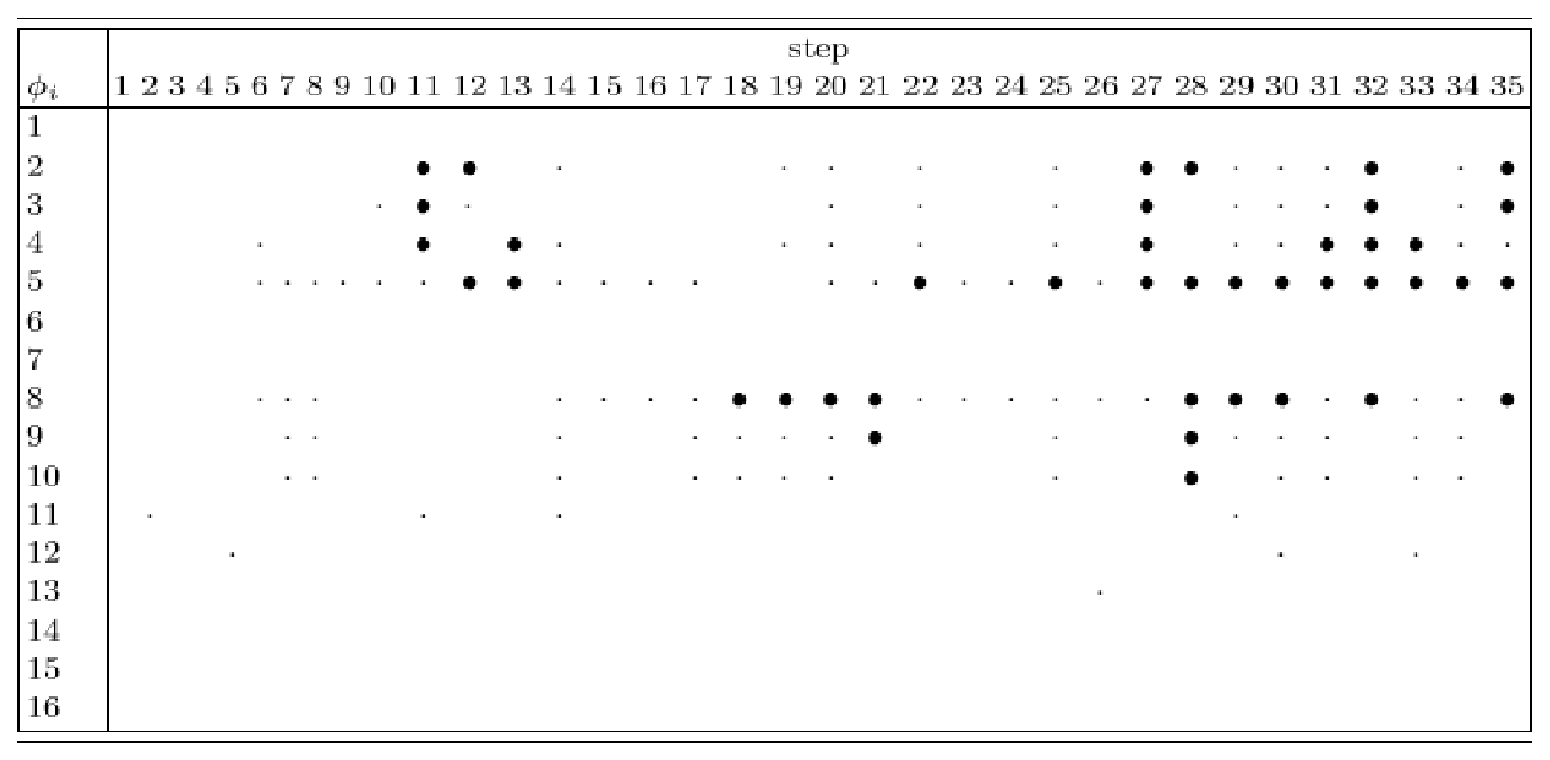
\includegraphics[width=0.49\columnwidth]{easytbl}
%\includegraphics[width=0.49\columnwidth]{hardtbl}
 \end{center}}
 \caption{Significant correlation (denoted by $\cdot$) for \easy (left) and \hard (right) problems and resulting ratio from optimality, $\rho$  defined by~\eqref{eq:ratio}. Commonly significant features across the tables are denoted by $\bullet$.}
 \label{tbl:feat:easynhard}
\end{table}

\section{Discussion and Conclusion}\label{sec:Discussion}

From the experimental study it is apparent that features have different %impact 
correlation with the resulting schedule depending in what stage it is in the scheduling process, implying that their influence varies throughout the scheduling process. And features constant throughout the scheduling process are not correlated with the end-result.
There are some common features for both difficulties considered which define JSSP on a whole. However the significant features are quite different across the two difficulties, implying there is a clear difference in their data structure. The amount of significant features were considerably more for easy problems, indicating their key elements had been found. However, the features distinguishing hard problems were scarce. Most likely due to their more complex data structure their key features are of a more composite nature.

%It is possible for a JSSP schedule to have more than one sequential dispatching representation. It is especially w.r.t. the initial dispatches. Visiting Fig.~\ref{fig:dispatch_example} again, if jobs \{1,2,3,6\} were to be dispatched first, then all permutations yield the same equivalent temporal schedule, this is because they don't create a conflict for one another. This drawback of non-uniqueness of sequential dispatching representation explains why there is hardly any significant feature for the initial steps of the scheduling process (cf. Table~\ref{tbl:feat:easynhard}). 

%Since feature selection is of paramount importance in order for algorithms to become successful, one needs to give great thought to how features are selected. What kind of features yield \bad schedules? And can they be steered onto the path of more promising feature characteristics. This sort of investigation can be an indicator how to create meaningful problem generators. On the account that real-world problem instances are scarce, their hidden properties need be drawn forth in order to generate artificial problem instances from the same data distribution. 

The feature attributes need to be based on statistical or theoretical grounds. Thus scrutiny in understanding the nature of problem instances is of paramount importance in feature engineering for learning. Which yields feedback into what features are important to devout more attention to, i.e. features that result in a failing algorithm. % For instance, in Table~\ref{tbl:feat:same} the slack features have the same distribution in the initial stages of the scheduling process, however there is a clear point of divergence which needs to be investigate why the sudden change? 
In general, this sort of investigation can undoubtedly be used in better algorithm design which is more equipped to deal with varying problem instances and tailor to individual problem instance's needs, i.e. a footprint-oriented algorithm. 

Although this methodology was only implemented on a simple single-priority dispatching rule heuristic, the methodology is easily adaptable for more complex algorithms. The main objective of this work is to illustrate the interaction of a specific algorithm on a given problem structure and its properties.
%The authors fully expect that this could help improve performance in solving JSSP with ordinal regression, which is a per-instance tuning paradigm. This is currently underway as an extension to work introduced in \cite{Ingimundardottir2010}.

% References to be used:
% \cite{Bouzarkouna2010}\cite{Hutter2006}\cite{Horvitz2001}\cite{Shahzad2010}\cite{Alanzi2006} 


\bibliographystyle{splncs}
\bibliography{lion6}

% that's all folks
\end{document}

